\chapter{Duality}
\label{chap:duality}

\section{LP duality*}
\label{sec:lp_duality}

Duality is fascinating topic in mathematical optimization: the basic arguments
used in the theory of duality are elementary and yet they can lead to powerful
and far-reaching conclusions.    

The story begins, for us, with linear programs (LPs). Consider a generic LP of
the form 
\begin{equation}
\label{eq:lp_primal}
\begin{alignedat}{2}
&\minimize_x \quad && c^\T x \\
&\st && Ax \leq b \\
& && Gx = h, 
\end{alignedat}
\end{equation}
where $c \in \R^d$, $A \in \R^{m \times d}$, $b \in \R^m$, $G \in \R^{k \times 
  d}$, $h \in \R^k$. The reason we start the chapter by studying LPs is that,   
in this problem class, we can build up dual problems ``constructively''; this 
constructive approach is not possible for general optimization problems, and
helps us appreciate the importance and elegance of Lagrange duality, which is
covered next.     

The fundamental question that underlies the study of duality is as follows: what
is the tightest lower bound we can form on the optimal criterion value $f^\star
= c^\T x^\star$ in \eqref{eq:lp_primal}? To address this, suppose that $u \in
\R^m$ and $v \in \R^k$ are arbitrary vectors---which we call \emph{dual 
  variables} in this context---with $u$ nonnegative in each component, $u \geq   
0$. Provided that $x \in \R^d$ is a feasible point for problem
\eqref{eq:lp_primal}, it holds that $u^\T (Ax - b) \leq 0$ and $v^\T (Gx - h) =
0$, and so, adding these together gives        
\begin{equation}
\label{eq:lp_dual_nonnegative}
u^\T (Ax - b) + v^\T (Gx - h) \leq 0.
\end{equation}
In order to obtain a lower bound on the criterion value $c^\T x$, we rearrange
the above into
\[
(-A^\T u - G^\T v)^\T x \geq -b^\T u - h^\T v.
\]
The key observation is that this provides the lower bound we desire provided
that the dual variables $u,v$ are chosen such that $-A^\T u - G^\T v= c$. This
is true for any feasible $x$, thus taking an infimum over all such $x$ gives   
\[
f^\star \geq -b^\T u - h^\T v, \quad \text{for any $u,v$ such that $-A^\T u -
  G^\T v = c$ and $u \geq 0$}.
\]
Finally, to make this lower bound as tight as possible, we maximize the
right-hand side above,  
\begin{equation}
\label{eq:lp_weak_duality}
f^\star \geq \, \underbrace{\sup \big\{ -b^\T u - h^\T v :  A^\T u + G^\T v =
  -c, \, u \geq 0 \big\}}_{g^\star}.
\end{equation}
Now the right-hand side in \eqref{eq:lp_weak_duality}, which we may denote as 
$g^\star = -b^\T u^\star - h^\T v^\star$, is itself the optimal criterion value
associated with an optimization problem, indeed an LP,     
\index{dual problem!linear program}
\begin{equation}
\label{eq:lp_dual}
\begin{alignedat}{2}
&\maximize_{u,v} \quad && b^\T u - h^\T v \\
&\st && A^\T u + G^\T v = -c \\
& && u \geq 0.
\end{alignedat}
\end{equation}
In this context, we call \eqref{eq:lp_dual} the \emph{dual LP} and the original 
problem \eqref{eq:lp_primal} the \emph{primal LP}. Note that, by construction 
\eqref{eq:lp_weak_duality}, we have $f^\star \geq g^\star$: the optimal
criterion in the dual problem is a lower bound on the optimal criterion in the  
primal problem.  

There are several natural follow-up questions that we can ask: for example, when
does equality hold in \eqref{eq:lp_weak_duality}, $f^\star = g^\star$? And, how 
do solutions $x^\star$ and $u^\star, v^\star$ in \eqref{eq:lp_primal} and
\eqref{eq:lp_dual}, respectively, relate? We will address these questions and
more, over this chapter and the next one. First, however, we must develop a
theory of duality beyond LPs. 

\begin{Remark}
In the attempt to move beyond LPs with the constructive approach to duality, we 
run into a shortcoming: when the criterion $f$ is nonlinear, but the constraint
functions are linear, we have no way in general to combine the
constraints---which are linear equalities and inequalities in $x$---to construct
a lower bound on $f(x)$. But there is another way: Lagrangian duality, as we
will see next, applies seamlessly to LPs and convex optimization more broadly
(and even some nonconvex problems).   
\end{Remark}

\section{Lagrangian duality}
\label{sec:lagrangian_duality}

Lagrangian duality (or Lagrange duality) starts with the same motivation as in
the last section, but cast in a more general setting: we seek a lower bound on
the optimal criterion value $f^\star$ in           
\begin{equation}
\label{eq:primal_problem}
\begin{alignedat}{2}
&\minimize_x \quad && f(x) \\
&\st \quad && h_i(x) \leq 0, \; i=1,\ldots,m \\ 
& && \ell_j(x) = 0, \; j=1,\ldots,k.
\end{alignedat}
\end{equation}
At the moment, we do not assume that criterion $f$ or the constraint functions
$h_i$, $i=1,\dots,m$, and $\ell_j$, $j=1,\dots,k$ are convex. Thus, to be clear,
we do not assume that \eqref{eq:primal_problem} is a convex problem. 

As before, let $u \in \R^m$ and $v \in \R^k$ be arbitrary vectors, with $u \geq
0$, which we call \emph{dual variables} in the current context. Using the same
basic idea as in \eqref{eq:lp_dual_nonnegative}, note that for any feasible $x$
for \eqref{eq:primal_problem}, 
\[
\sum_{i=1}^m u_i h_i(x) + \sum_{j=1}^r v_j \ell_j(x) \leq 0.
\]
We now add this quantity to the criterion $f(x)$ to define what we call the
\emph{Lagrangian function},   
\index{Lagrangian function}
\[
L(x,u,v) = f(x) + \sum_{i=1}^m u_i h_i(x) + \sum_{j=1}^r v_j \ell_j(x).
\] 
By construction, this provides a lower bound on the criterion,
\begin{equation}
\label{eq:lagrangian_lb1}
f(x) \geq L(x,u,v), \quad \text{for any feasible $x$ and $u,v$ such that $u
  \geq 0$},
\end{equation}
and minimizing over the feasible set, denoted $C \subseteq \R^d$, yields
\begin{equation}
\label{eq:lagrangian_lb2}
f^\star \geq \inf_{x \in C} \, L(x,u,v) \geq \inf_x \, L(x,u,v), \quad \text{for
  any $u,v$ such that $u \geq 0$}.  
\end{equation}

\begin{Remark}
The second inequality in \eqref{eq:lagrangian_lb2} is really the key idea behind
Lagrangian duality; had we stopped at the first inequality in
\eqref{eq:lagrangian_lb2}, we would have not have (yet) gotten anywhere
practically interesting, since minimizing the Lagrangian over $x \in C$ is  
hard in general---it is no easier than minimizing $f$ over $x \in C$, which is
our original primal problem \eqref{eq:primal_problem}. Meanwhile, minimizing the
Lagrangian over $x \in \R^d$ is usually more tractable (as we will see in 
examples that follow), and still produces an effective lower bound.
\end{Remark}

It is convenient to denote the right-most quantity in \eqref{eq:lagrangian_lb2}
by 
\index{dual function}
\begin{equation}
\label{eq:dual_function}
g(u,v) = \inf_x \, L(x,u,v), 
\end{equation}
which we call the \emph{Lagrange dual function}. Then \eqref{eq:lagrangian_lb2}
reads $f^\star \geq g(u,v)$ for any $u,v$ with $u \geq 0$, and we can maximize
$g$ to obtain the tightest lower bound, yielding 
\index{dual problem}
\begin{equation}
\label{eq:dual_problem}
\maximize_{u,v} \quad g(u,v) \quad \st \quad u \geq 0,
\end{equation}
which we call the \emph{Lagrange dual problem} associated with
\eqref{eq:primal_problem}. Our convention will be to drop the term ``Lagrange''
when referring to the dual function and dual problem defined above.

\begin{Example}
In what follows, we work through the duals of canonical problems: LPs and
QPs. For the duals standard form LPs and QPs, see Exercises \ref{ex:lp_std_dual}
and \ref{ex:qp_std_dual}.   

\begin{enumerate}[label=\alph*., ref=\alph*]
\item \parlab{xa:lp_dual} 
For the linear program \eqref{eq:lp_primal}, the Lagrangian is
\begin{align*}
L(x,u,v) &= c^\T x + u^\T (Ax - b) + v^\T (Gx - h) \\
&= (c + A^\T u + G^\T v)^\T x - b^\T u - h^\T v.
\end{align*}
The dual function is obtained by taking an infimum over all $x$,
\[
g(u,v) = 
\begin{cases}
- b^\T u - h^\T v & A^\T u + G^\T v = -c \\
- \infty & \text{otherwise}.
\end{cases}
\]
The dual problem, which maximizes $g(u,v)$ subject to the constraint $u \geq
0$, is therefore precisely as derived earlier in \eqref{eq:lp_dual}. 

\item \parlab{xa:qp_dual}
For the quadratic program (QP): 
\begin{equation}
\label{eq:qp_primal}
\begin{alignedat}{2}
&\minimize_x \quad && \frac{1}{2} x^\T Q x + c^\T x\\ 
&\st && Ax \leq b \\
& && Gx = h,
\end{alignedat}
\end{equation}
the Lagrangian is
\begin{align*}
L(x,u,v) &= \frac{1}{2} x^\T Q x + c^\T x + u^\T (Ax - b) + v^\T (Gx - h) \\ 
&= \frac{1}{2} x^\T Q x + (c + A^\T u + G^\T v)^\T x - b^\T u - h^\T v. 
\end{align*}
Assume that $Q \succ 0$. We can minimize the Lagrangian over $x$ by setting its
gradient to zero and solving, which yields $x = - Q^{-1} (c + A^\T u + G^\T v)$,
and   
\[
g(u,v) = - \frac{1}{2} (c + A^\T u + G^\T v)^\T Q^{-1} (c + A^\T u + G^\T v) -
b^\T u - h^\T v.
\] 
The dual problem is thus
\index{dual problem!quadratic program}
\begin{equation}
\label{eq:qp_pd_dual}
\begin{alignedat}{2}
&\maximize_{u,v} \quad && - \frac{1}{2} (c + A^\T u + G^\T v)^\T Q^{-1} (c +
A^\T u + G^\T v) - b^\T u - h^\T v \\
&\st && u \geq 0.
\end{alignedat}
\end{equation}
This is itself a QP. If instead $Q \succeq 0$, then similar arguments (Exercise
\ref{ex:qp_psd_dual}) lead to  
\begin{equation}
\label{eq:qp_psd_dual}
\begin{alignedat}{2}
&\maximize_{u,v} \quad && - \frac{1}{2} (c + A^\T u + G^\T v)^\T Q^\pinv (c + 
A^\T u + G^\T v) - b^\T u - h^\T v \\
&\st && c + A^\T u + G^\T v \in \col(Q) \\ 
& && u \geq 0.
\end{alignedat}
\end{equation}
This is still a QP, because $c + A^\T u + G^\T v \in \col(Q)$ (where $\col(Q)$
denotes the column space of $Q$) is a linear constraint.    
\end{enumerate}
\end{Example}

\section{Properties}

Next we cover two important properties of Lagrange duality, which follow
more or less immediately from the development in the last section.

\paragraph{Weak duality.}
\parlab{par:weak_duality}

Let $g^\star$ denote the optimal value in the dual problem
\eqref{eq:dual_problem}. It follows from \eqref{eq:lagrangian_lb2} and the  
definition of the dual function in \eqref{eq:dual_function} that  
\index{weak duality}
\begin{equation}
\label{eq:weak_duality}
f^\star \geq g^\star.
\end{equation}
This property is called \emph{weak duality}, and it holds for \emph{any}
original (primal) problem \eqref{eq:primal_problem}, regardless of
convexity. Note that this generalizes what we found in
\eqref{eq:lp_weak_duality} for LPs. 

\paragraph{Convexity of dual problem.}
\parlab{par:convex_dual}

The dual optimization problem \eqref{eq:dual_problem} is \emph{always convex},
that is, it is a concave maximization problem. This is true for any original
(primal) problem \eqref{eq:primal_problem}, regardless of whether the primal
problem is itself convex. To see this, we can rewrite the dual function
\eqref{eq:dual_function} as   
\[
g(u,v) = - \, \underbrace{\sup_x \, \bigg\{ -f(x) - \sum_{i=1}^m u_i h_i(x) - 
  \sum_{j=1}^r v_j \ell_j(x) \bigg\}}_{\bar{g}(u,v)}.
\]
Observe that the function defined as \smash{$\bar{g}$} above is the pointwise 
supremum of affine---hence convex---functions in $u,v$. By the pointwise
supremum rule in Property \parref{par:function_supremum}, we see that
\smash{$\bar{g}$} is convex, and therefore the dual function \smash{$g =
  -\bar{g}$} is concave. This makes problem \eqref{eq:dual_problem} convex.     

\medskip

\begin{Example}
The following example emphasizes how Property \parref{par:convex_dual} can be
surprising and nonobvious in practice. Consider the nonconvex optimization
problem 
\[
\minimize_x \quad \frac{1}{10} x^4 - 5x^2 + 10x + 15 \quad \st \quad x \geq -4. 
\]
The left panel of Figure \ref{fig:nonconvex_quartic} plots its criterion, which
is a nonconvex quartic function. Despite such nonconvexity, we can calculate the
dual function for this problem explicitly because it reduces to solving for the
roots of a cubic equation, which can be done in closed-form. Some calculations
(Exercise \ref{ex:nonconvex_quartic}) lead to:
\[
g(u) = \min_{j=1,2,3} \, \bigg\{ \frac{1}{10} F_j^4(u) - 5 F_j^2(u) + 10 F_j(u)
+ 15 \bigg\},
\]
where 
\[
F_j(u) = ..., \quad j = 1,2,3,
\]
and $a_1 = 1$, \smash{$a_2 = (-1 + i \sqrt{3})/2$}, and \smash{$a_3 = (-1 - i 
  \sqrt{3})/2$} (with $i$ here denoting the imaginary unit). The right panel of
Figure \ref{fig:nonconvex_quartic} plots the dual criterion; that this function
is concave, as guaranteed by Property \parref{par:convex_dual}, is not at all 
obvious from its analytic form!  
\end{Example}

\begin{figure}[tb]
\centering
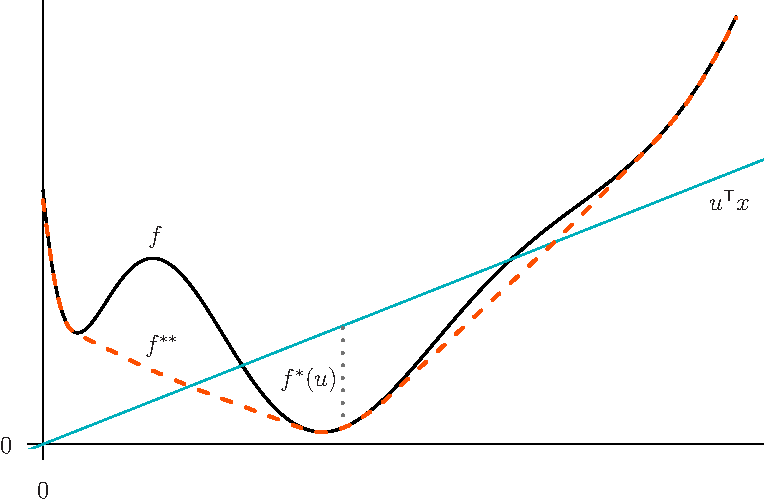
\includegraphics[width=0.7\textwidth]{fig/conjugate.pdf}
\caption{The conjugate $f^*$ evaluated at $u$ is the maximum gap between a
  linear function with slope $u$ and $f$, illustrated by the dotted line. The
  double conjugate $f^{**}$ is the pointwise supremum of all affine minorants to
  $f$ (equivalently, the greatest closed convex minorant to $f$), illustrated by
  the dashed line.}     
\label{fig:nonconvex_quartic}
\end{figure}

\section{Interpretations}
\label{sec:duality_interpretations}

\section{Slater's condition}
\label{sec:slater_condition}

\section{SDP duality*}
\label{sec:sdp_duality}

% for SDP duality: take a look at 
% https://www.mit.edu/~parrilo/cdc03_workshop/ejc03_comp.pdf
% https://ocw.mit.edu/courses/electrical-engineering-and-computer-science/6-251j-introduction-to-mathematical-programming-fall-2009/readings/MIT6_251JF09_SDP.pdf

\SkipTocEntry\section*{Chapter notes}

\clearpage

\begin{xcb}{Exercises}
\begin{enumerate}[label=\thechapter.\arabic*]
\settowidth{\leftmargini}{0.00.\hskip\labelsep}

\item \label{ex:lp_std_dual}
Standard form LP dual

\item \label{ex:qp_std_dual} 
Standard form QP dual

\item \label{ex:qp_psd_dual} 
PSD QP dual

\item \label{ex:nonconvex_quartic}
Nonconvex quartic

\item 

\end{enumerate}
\end{xcb}
